% Generated by benchmark/fig4_options.py (option 3, chosen by the authors) -- do not edit by hand.
\begin{figure}[t]
\centering
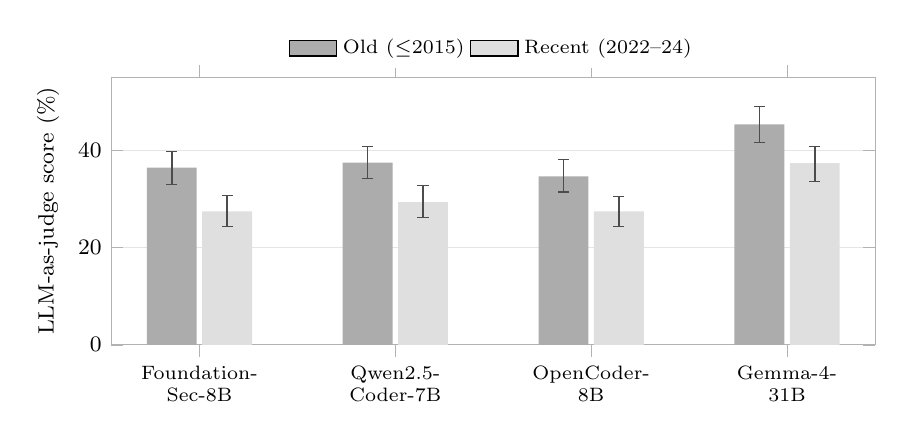
\begin{tikzpicture}
\begin{axis}[scale only axis, width=0.80\columnwidth, height=3.4cm, ybar=2pt, bar width=18pt, ymin=0, ymax=55,
  xtick={0,1,2,3}, xticklabels={{Foundation-\\Sec-8B},{Qwen2.5-\\Coder-7B},{OpenCoder-\\8B},{Gemma-4-\\31B}}, enlarge x limits=0.15,
  x tick label style={font=\scriptsize, align=center}, y tick label style={font=\footnotesize}, ylabel={\footnotesize LLM-as-judge score (\%)},
  ymajorgrids, grid style={gray!20}, axis line style={gray!60}, tick style={gray!60},
  legend style={font=\scriptsize, at={(0.5,1.03)}, anchor=south, draw=none}, legend columns=2, area legend]
\addplot[fill=gray!65, draw=none, error bars/.cd, y dir=both, y explicit, error bar style={line width=0.6pt, black!70}] coordinates {(0,36.4) -= (0,3.4) += (0,3.3) (1,37.4) -= (0,3.3) += (0,3.4) (2,34.6) -= (0,3.2) += (0,3.4) (3,45.3) -= (0,3.7) += (0,3.6)};
\addlegendentry{Old ($\leq$2015)}
\addplot[fill=gray!25, draw=none, error bars/.cd, y dir=both, y explicit, error bar style={line width=0.6pt, black!70}] coordinates {(0,27.4) -= (0,3.1) += (0,3.2) (1,29.3) -= (0,3.2) += (0,3.4) (2,27.4) -= (0,3.1) += (0,3.1) (3,37.3) -= (0,3.7) += (0,3.5)};
\addlegendentry{Recent (2022--24)}
\end{axis}
\end{tikzpicture}
\caption{Judge score on old ($\leq$2015, 357 records) and recent (2022--2024, 325 records) CVEs, CVEfixes test
records only. Error bars are 95\% bootstrap intervals over records. Scores in the intermediate years fluctuate
(Section~\ref{sec:benchmark-results}).}
\label{fig:memorisation}
\end{figure}
